\documentclass{beamer}
\usepackage[latin1]{inputenc}
\usepackage{color}
\usepackage[absolute,overlay]{textpos} 
\usetheme{Warsaw}

\expandafter\def\expandafter\insertshorttitle\expandafter{%\insertshorttitle\hfill%
  \insertframenumber\,/\,\inserttotalframenumber}

\definecolor{red}{rgb}{1,0,0}
\title[TagFS]{A tag based filesystem}
\author{Catalina Macalet, Eugen Hristev, Mihai Dinu, Sorin Dumitru}
\institute{Politehnic University of Bucharest}
\date{Nov 11, 2010}
\begin{document}

\begin{frame}
  \titlepage
\end{frame}

\section{Choices}

\begin{frame}{Where we left off}
    \begin{itemize}
        \item{VFS changes or new fs}
        \item{Metadata storage}
	\item{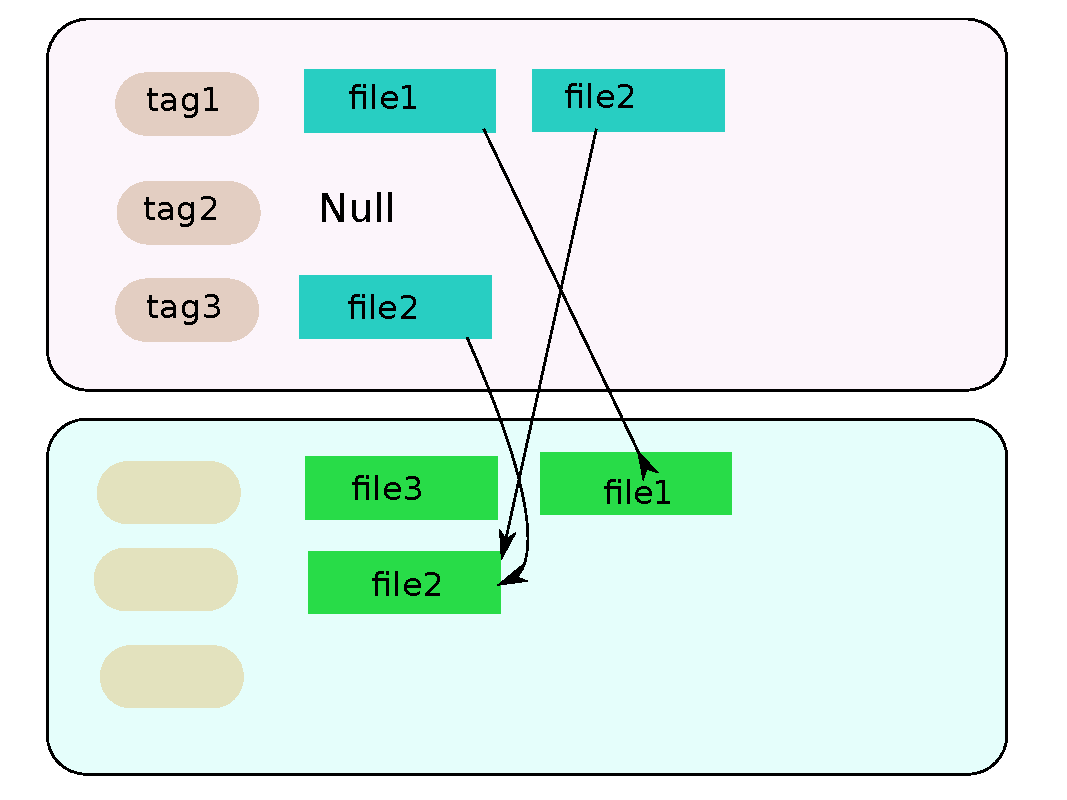
\includegraphics[scale=0.4]{poza.pdf}}
    \end{itemize}
\end{frame}

\begin{frame}{Assumptions}
    \begin{itemize}
        \item{Do as few changes as possible}
        \item{Filename separated from tags by ":"}
        \item{Limit the length of filename and/or tags to MAX$\_$PATH}
        \item{Define tagfs start points in file system hierarchy}
        \item{Store the tagfs metadata files in RAM}
    \end{itemize}
\end{frame}

\section{Operations}

\begin{frame}{VFS Operations}
    \begin{itemize}
        \item \textcolor{red}{touch filename:tag1:tag2:...}
            \begin{itemize}
                \item{create file with tags (add metadata in tagfs structure)}
                \item{vfs function: do$\_$sys$\_$open}
            \end{itemize}
        \item \textcolor{red}{mv}
            \begin{itemize}
                \item{move file (change metadata in tagfs structure)}
                \item{vfs function: rename}
            \end{itemize}
        \item \textcolor{red}{cp}
            \begin{itemize}
                \item{create a copy of file (add metadata in tagfs structure)}
                \item{vfs function: unlink}
            \end{itemize}
        \item \textcolor{red}{ls}
            \begin{itemize}
                \item{list files and associated tags, iterate through tagfs structure}
                \item{vfs function: getdents}
            \end{itemize}
    \end{itemize}
\end{frame}

\begin{frame}{New Operations}
    \begin{itemize}
        \item {All use fcntl syscall}
        \item \textcolor{red}{ tag -l filename}
            \begin{itemize}
                \item{list tags associated with a file}
            \end{itemize}
        \item \textcolor{red}{ tag -a filename:tag1:tag2:...}
            \begin{itemize}
                \item{Add tag1, tag2,.. tags to file}
            \end{itemize}
        \item \textcolor{red}{ tag -d filename:tag1:tag2:...}
            \begin{itemize}
                \item{Remove tag1, tag2,... tags from file}
            \end{itemize}
    \end{itemize}
\end{frame}

\section{Status}
\begin{frame}{Current status}
    \begin{itemize}
        \item {Implemented structure for storing metadata}
        \item {Testing tool for storage module}
        \item {Userspace tool for add/remove/list tags}
        \item {Hacks in vfs}
    \end{itemize}
\end{frame}

\begin{frame}{TODOs}
    \begin{itemize}
        \item {Further testing for storage module}
        \item {Implement kernelspace side for user-tool}
        \item {More hacks in vfs}
    \end{itemize}
\end{frame}

\end{document}
